\documentclass{article}
\usepackage[utf8x]{inputenc}
\usepackage{amsmath}
\usepackage{algorithm}
\usepackage{algorithmicx}
\usepackage{fancyvrb}
\usepackage{verbatim}
\usepackage[noend]{algpseudocode}
\usepackage{mathtools}
\newcommand*\Let[2]{\State #1 $\gets$ #2}
\algrenewcommand\algorithmicrequire{\textbf{Precondition:}}
\algrenewcommand\algorithmicensure{\textbf{Postcondition:}}
\title{Laboratorio 4 - Redes e programação Linear}
\author{Gabriel Hidasy Rezende, RA116928}
\begin{document}
\maketitle
\section*{Problema}
\paragraph{} Dado um grafo $G = (V,E)$, uma função de latência das
arestas $l:E \rightarrow R^+$, uma função de capacidade das arestas
$d: E \rightarrow R^+$, uma função do custo das arestas
$c: E \rightarrow R^+$ e uma lista de $k$ elementos
$P={(s_1,t_1,q_1,T_1),(s_2,t_2,q_2,T_2)...}$ onde cada elemento indica que o
nó $s_i$ quer transmitir $q_i$ dados para $t_i$ em tempo $\le T_i$ (ie
$T_i \le \sum{e} \quad \forall \, e\, \text{caminho}(s_i,t_i)$.
\paragraph{} Um detalhe que distingue esse problema do fluxo máximo é
que consideramos os dados $q_i$ indivisíveis, isso é, eles devem
trafegar todos pelo mesmo caminho
\section*{Estrategia}
\paragraph{} Será usada programação linear inteira. O problema
consiste em encontrar uma série de caminhos de 
tal que todas as restrições sejam satisfeitas.
\subparagraph{} Começando com a formulação base do problema de
caminhos mínimos:
\begin{align*}
  \text{Minimize} \sum_{ij}{c_{ij}x_{ij}} \quad (i,j) \in E
\end{align*}
\paragraph{} Sujeito a:
\begin{eqnarray*}
  \sum{x_{ij}-x_{ji}} &=& 1 \rightarrow i =s\\
  &=& -1 \rightarrow i = t\\
  &=& 0 \rightarrow i = \text{Others}
\end{eqnarray*}
\paragraph{} Adicionamos ao modelo as restrições de latência e
capacidade, e adicionando o numero de bits a função de minimização.
\begin{align*}
  \text{Minimize} \sum_{ij}{c_{ij}x_{ij}q} \quad (i,j) \in E
\end{align*}
\paragraph{} Sujeito a:
\begin{align*}
  \sum{x_{ij}+x_{ji}} \le T\\
  \forall (i,j) (x_{ij}+x_{ji})q \le w_{ij}\\
\end{align*}
\paragraph{} E finalmente generalizando a tarefa para n pares
\begin{align*}
  \text{Minimize} &\sum_{z}{\sum_{ij}{c_{ij}x_{ijz}q_z}}& \quad (i,j) \in E
\end{align*}
\paragraph{} Sujeito a:
\begin{align*}
  \forall z \sum{(x_{ijz}+x_{jiz})l_{ij}} &\le& T_z\\
  \forall (i,j) \sum{(x_{ijz}+x_{jiz})q_z} &\le& w_{ij}\\
  \forall z \sum{x_{ijz}-x_{jiz}} &=& 1 \rightarrow i=z(s)\\
  &=& -1 \rightarrow i = z(t)\\
  &=& 0 \rightarrow \text{Others}\\
\end{align*}
\section*{Implementação}
\paragraph{} Segue no anexo.
\section*{Experimentos}
\paragraph{} Para os experimentos usei o gerador disponibilizado para
criar um conjunto de entradas, tanto de entradas onde o gerador podia
fornecer uma solução ótima quanto para problemas sem ótimo
conhecido. Para os problemas com ótimo conhecido a resposta sempre foi
próxima (exata até a terceira casa decimal) da ótima conhecida devido
a erros de arredondamento.
\paragraph{} O programa foi testado contra entradas com tamanho
variando de 100 a 2000 nós e de 5 a 50 conexões para os testes com
resposta ótima conhecida, e de 100 até 450 nós de 5 até 50 conexões
(É interessante notar o caso com 45 conexões e 100 nós, que foi um
caso onde o programa demorou MUITO mais do que o esperado para
resolver o problema (470s), no gráfico substitui o mesmo por 12 para
não achatar os demais)


\section*{Resultados} Seguem abaixo as tabelas com os tempos coletados
para cada execução do programa com entradas conhecidas:
\begin{center}
\begin{tabular}{rrrrrrrrr}
n/p & 100 & 400 & 700 & 1000 & 1300 & 1600 & 1900 & 2000\\
5 & 0.050887 & 0.17113 & 0.36009 & 0.62692 & 1.08667 & 1.16733 & 1.25892 & 1.95130\\
10 & 0.109931 & 0.41025 & 1.11885 & 1.30583 & 2.63491 & 2.91770 & 4.29974 & 4.10567\\
15 & 0.169644 & 0.68096 & 1.38437 & 2.54122 & 2.99534 & 4.61477 & 6.11132 & 6.73419\\
20 & 0.231992 & 1.35648 & 2.72076 & 3.16017 & 4.55223 & 8.73329 & 8.01861 & 8.17655\\
25 & 0.295344 & 1.31960 & 3.03287 & 4.27775 & 9.36292 & 10.0769 & 13.2401 & 15.7380\\
30 & 0.346487 & 1.88953 & 3.72942 & 7.15288 & 6.80763 & 9.21231 & 18.3581 & 14.1724\\
35 & 0.453721 & 2.49261 & 4.98895 & 6.64401 & 11.7983 & 15.0093 & 17.2614 & 18.6811\\
40 & 0.539139 & 2.89146 & 4.33689 & 8.30682 & 12.6869 & 18.3852 & 19.6628 & 22.1970\\
45 & 0.575044 & 3.53962 & 6.28981 & 12.0244 & 19.6412 & 26.3799 & 27.8474 & 24.0224\\
50 & 0.663847 & 3.55586 & 5.95327 & 11.5242 & 19.5810 & 22.2215 & 28.6196 & 28.8540\\
\end{tabular}
\end{center}
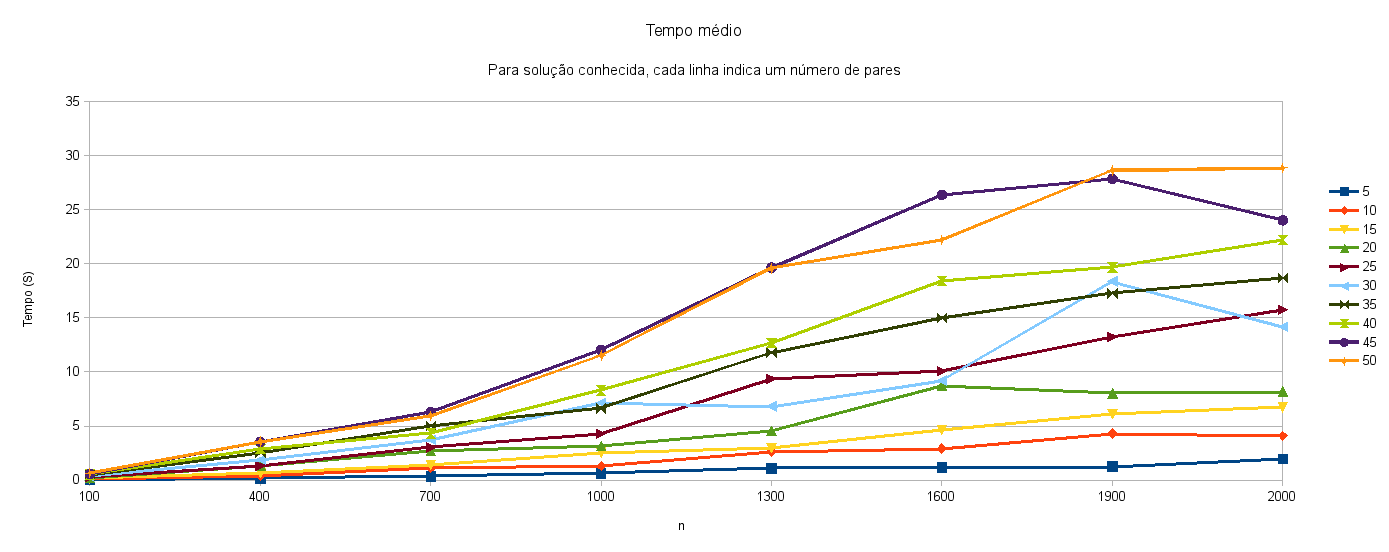
\includegraphics[scale=0.4]{graphic_know}
\paragraph{} E a mesma tabela repetida em casos sem a solução
conhecida, nesse caso o tamanho dos problemas é bem menor para
permitir que o programa termine em um tempo razoável.
\begin{center}
\begin{tabular}{rrrrrrrrr}
n/p & 100 & 150 & 200 & 250 & 300 & 350 & 400 & 450 \\
5  & 0.05444 & 0.32642 & 0.27151 & 0.10360 & 0.07055 & 0.23850 & 0.25654 & 0.12259 \\
10 & 0.08720 & 0.75095 & 0.75788 & 0.58290 & 1.26851 & 0.41367 & 1.39200 & 0.58620\\
15 & 0.16639 & 0.81763 & 0.99769 & 1.67869 & 1.86789 & 0.72099 & 2.27418 & 1.02499\\
20 & 0.43913 & 1.39768 & 1.67676 & 2.06044 & 3.13629 & 1.29749 & 5.28618 & 1.49889\\
25 & 0.49088 & 1.68882 & 1.75044 & 3.74337 & 1.97310 & 1.63258 & 4.22772 & 2.68861\\
30 & 0.72422 & 3.57542 & 2.52983 & 5.09696 & 4.03528 & 3.59689 & 4.50125 & 3.77938\\
35 & 1.44865 & 2.62594 & 2.40432 & 6.12104 & 5.60085 & 3.39431 & 9.89985 & 3.88167\\
40 & 11.1556 & 8.03197 & 8.41365 & 7.77423 & 13.0921 & 6.06245 & 10.9787 & 12.2957\\
45 & 740.516 & 3.27903 & 11.3131 & 7.69732 & 7.37726 & 8.92662 & 7.67648 & 12.5595\\
50 & 15.3100 & 15.2817 & 11.1226 & 8.21201 & 22.8836 & 6.72498 & 9.32185 & 15.5944\\
\end{tabular}
\end{center}
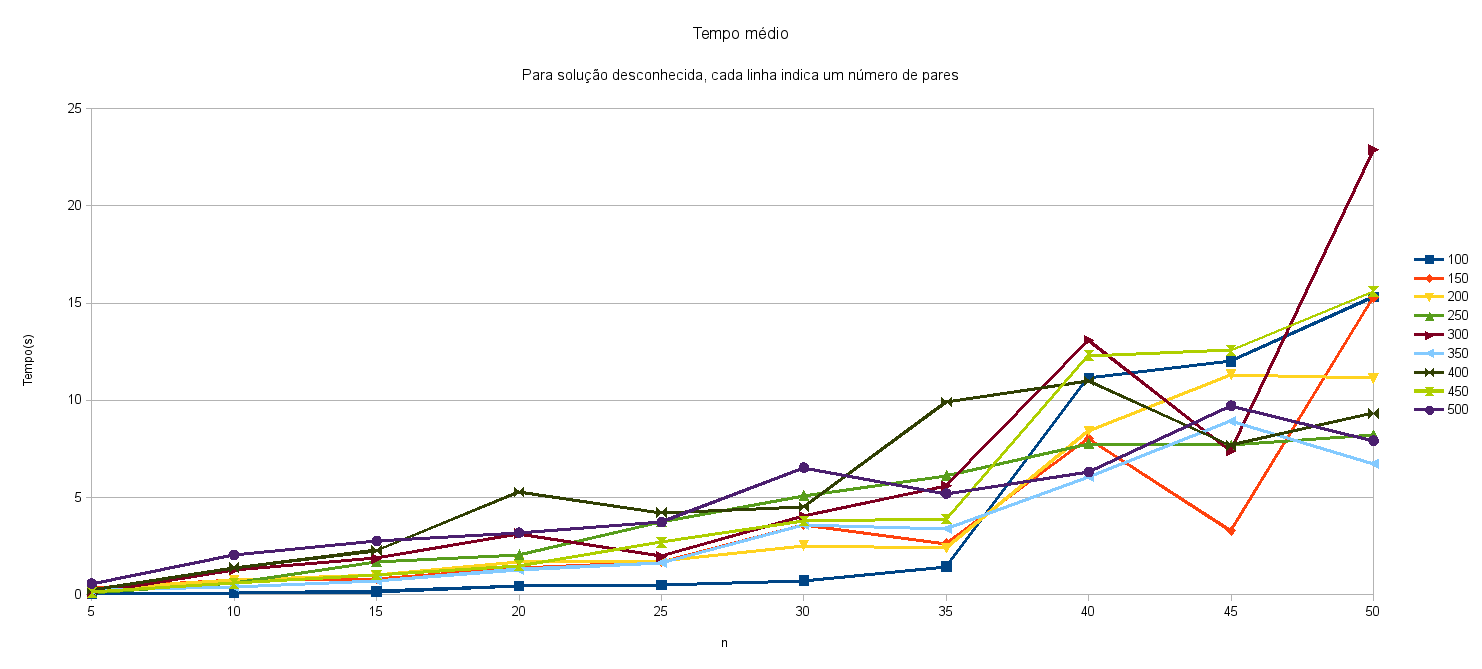
\includegraphics[scale=0.4]{graphic_unknow}
\end{document}
